\documentclass[fontset=windows]{article}
\usepackage[margin=1in]{geometry}%设置边距,符合Word设定
\usepackage{ctex}
\usepackage{amsmath, xparse}
\usepackage{amssymb}
\usepackage{setspace}
\usepackage{lipsum}
\usepackage{graphicx}%插入图片
\usepackage{multirow}%多列表格
\graphicspath{{Figures/}}%文章所用图片在当前目录下的 Figures目录
\usepackage{hyperref} % 对目录生成链接,注:该宏包可能与其他宏包冲突,故放在所有引用的宏包之后
\hypersetup{
    colorlinks        = true,  % 将链接文字带颜色
	bookmarksopen     = true, % 展开书签
	bookmarksnumbered = true, % 书签带章节编号
	pdftitle          = 标题, % 标题
	pdfauthor         = DarkSharpness, % 作者
    citecolor         = green,
    linkcolor         = black,
    urlcolor          = blue
}
\bibliographystyle{plain}% 参考文献引用格式
\newcommand{\upcite}[1]{\textsuperscript{\cite{#1}}}

\renewcommand{\contentsname}{\centerline{Contents}} %经过设置word格式后,将目录标题居中

% Keywords command
\providecommand{\keywords}[1]
{
  \textbf{\text{Keywords: }} #1
}

\title{\heiti\zihao{2} 光盘彩色线现象研究}
\author{DarkSharpness}
\date{2023.06.17}

\begin{document}
	\maketitle
	% \thispagestyle{empty}

摘要
\begin{abstract} 
    当光盘接受来自灯的光线照射后,表面可以清晰地看到一条彩色的亮线。我们对这一现象进行了理论解释,并设计实验与理论计算进行比对。
\end{abstract}

\keywords{光栅}

\tableofcontents

% 这是图片
% Hello world! Hello Ali! As shown in figure \ref{1}
% \begin{figure}[htbp]
% 	\centering
% 	\includegraphics[scale=0.2]{Ali.jpg}
% 	\caption{this is Ali}
% 	\label{1}
% \end{figure}

\section{引言}

CD 和 DVD 是广泛使用的光学存储介质,利用光的反射和衍射原理进行数据的存储和读取。这些光盘由聚碳酸酯基片、具有反射性金属层(通常是铝)和保护涂层组成。反射层包含一条螺旋状的凹坑和平地轨迹,代表二进制信息,如图1所示。

\begin{figure}[htbp]
	\centering
	\includegraphics[scale=0.6]{1.png}
	\caption{光盘轴面剖面局部放大图}
	\label{1}
\end{figure}

当光照射到 CD 或 DVD 表面的时候,我们常常可以观察到其表面出现彩色的光,如图2所示。

\begin{figure}[htbp]
	\centering
	\includegraphics[scale=0.05]{lines.jpg}
	\caption{CD 在白光台灯照射下的照片}
	\label{2}
\end{figure}

当白光从不同的角度入射,在不同的角度观察,我们可以看到不同颜色的彩色线,而颜色在光盘上的分布位置也会随之改变。这种现象可能的一种解释是,CD 和 DVD 表面的凹坑和平地呈周期性排布,构成了类似反射光栅的光学结构。由于光的衍射,不同颜色的光在空间中有不同的光强分布,因此在不同位置,我们能观察到不同颜色的光。

为了研究这一现象,我们将固定入射角度,并观察不同角度观察到的颜色。通过分析实验数据,确定反射角度和观察到的颜色之间的模式和相关性。此外,我们建立了理论模型来定量计算衍射效应,用实验验证该模型,进而对现象做出合理的解释。

\section{实验原理}

CD 和 DVD 表面的凹坑和平地围绕圆心,沿半径方向呈周期性排布,如图3所示。

\begin{figure}[htbp]
	\centering
	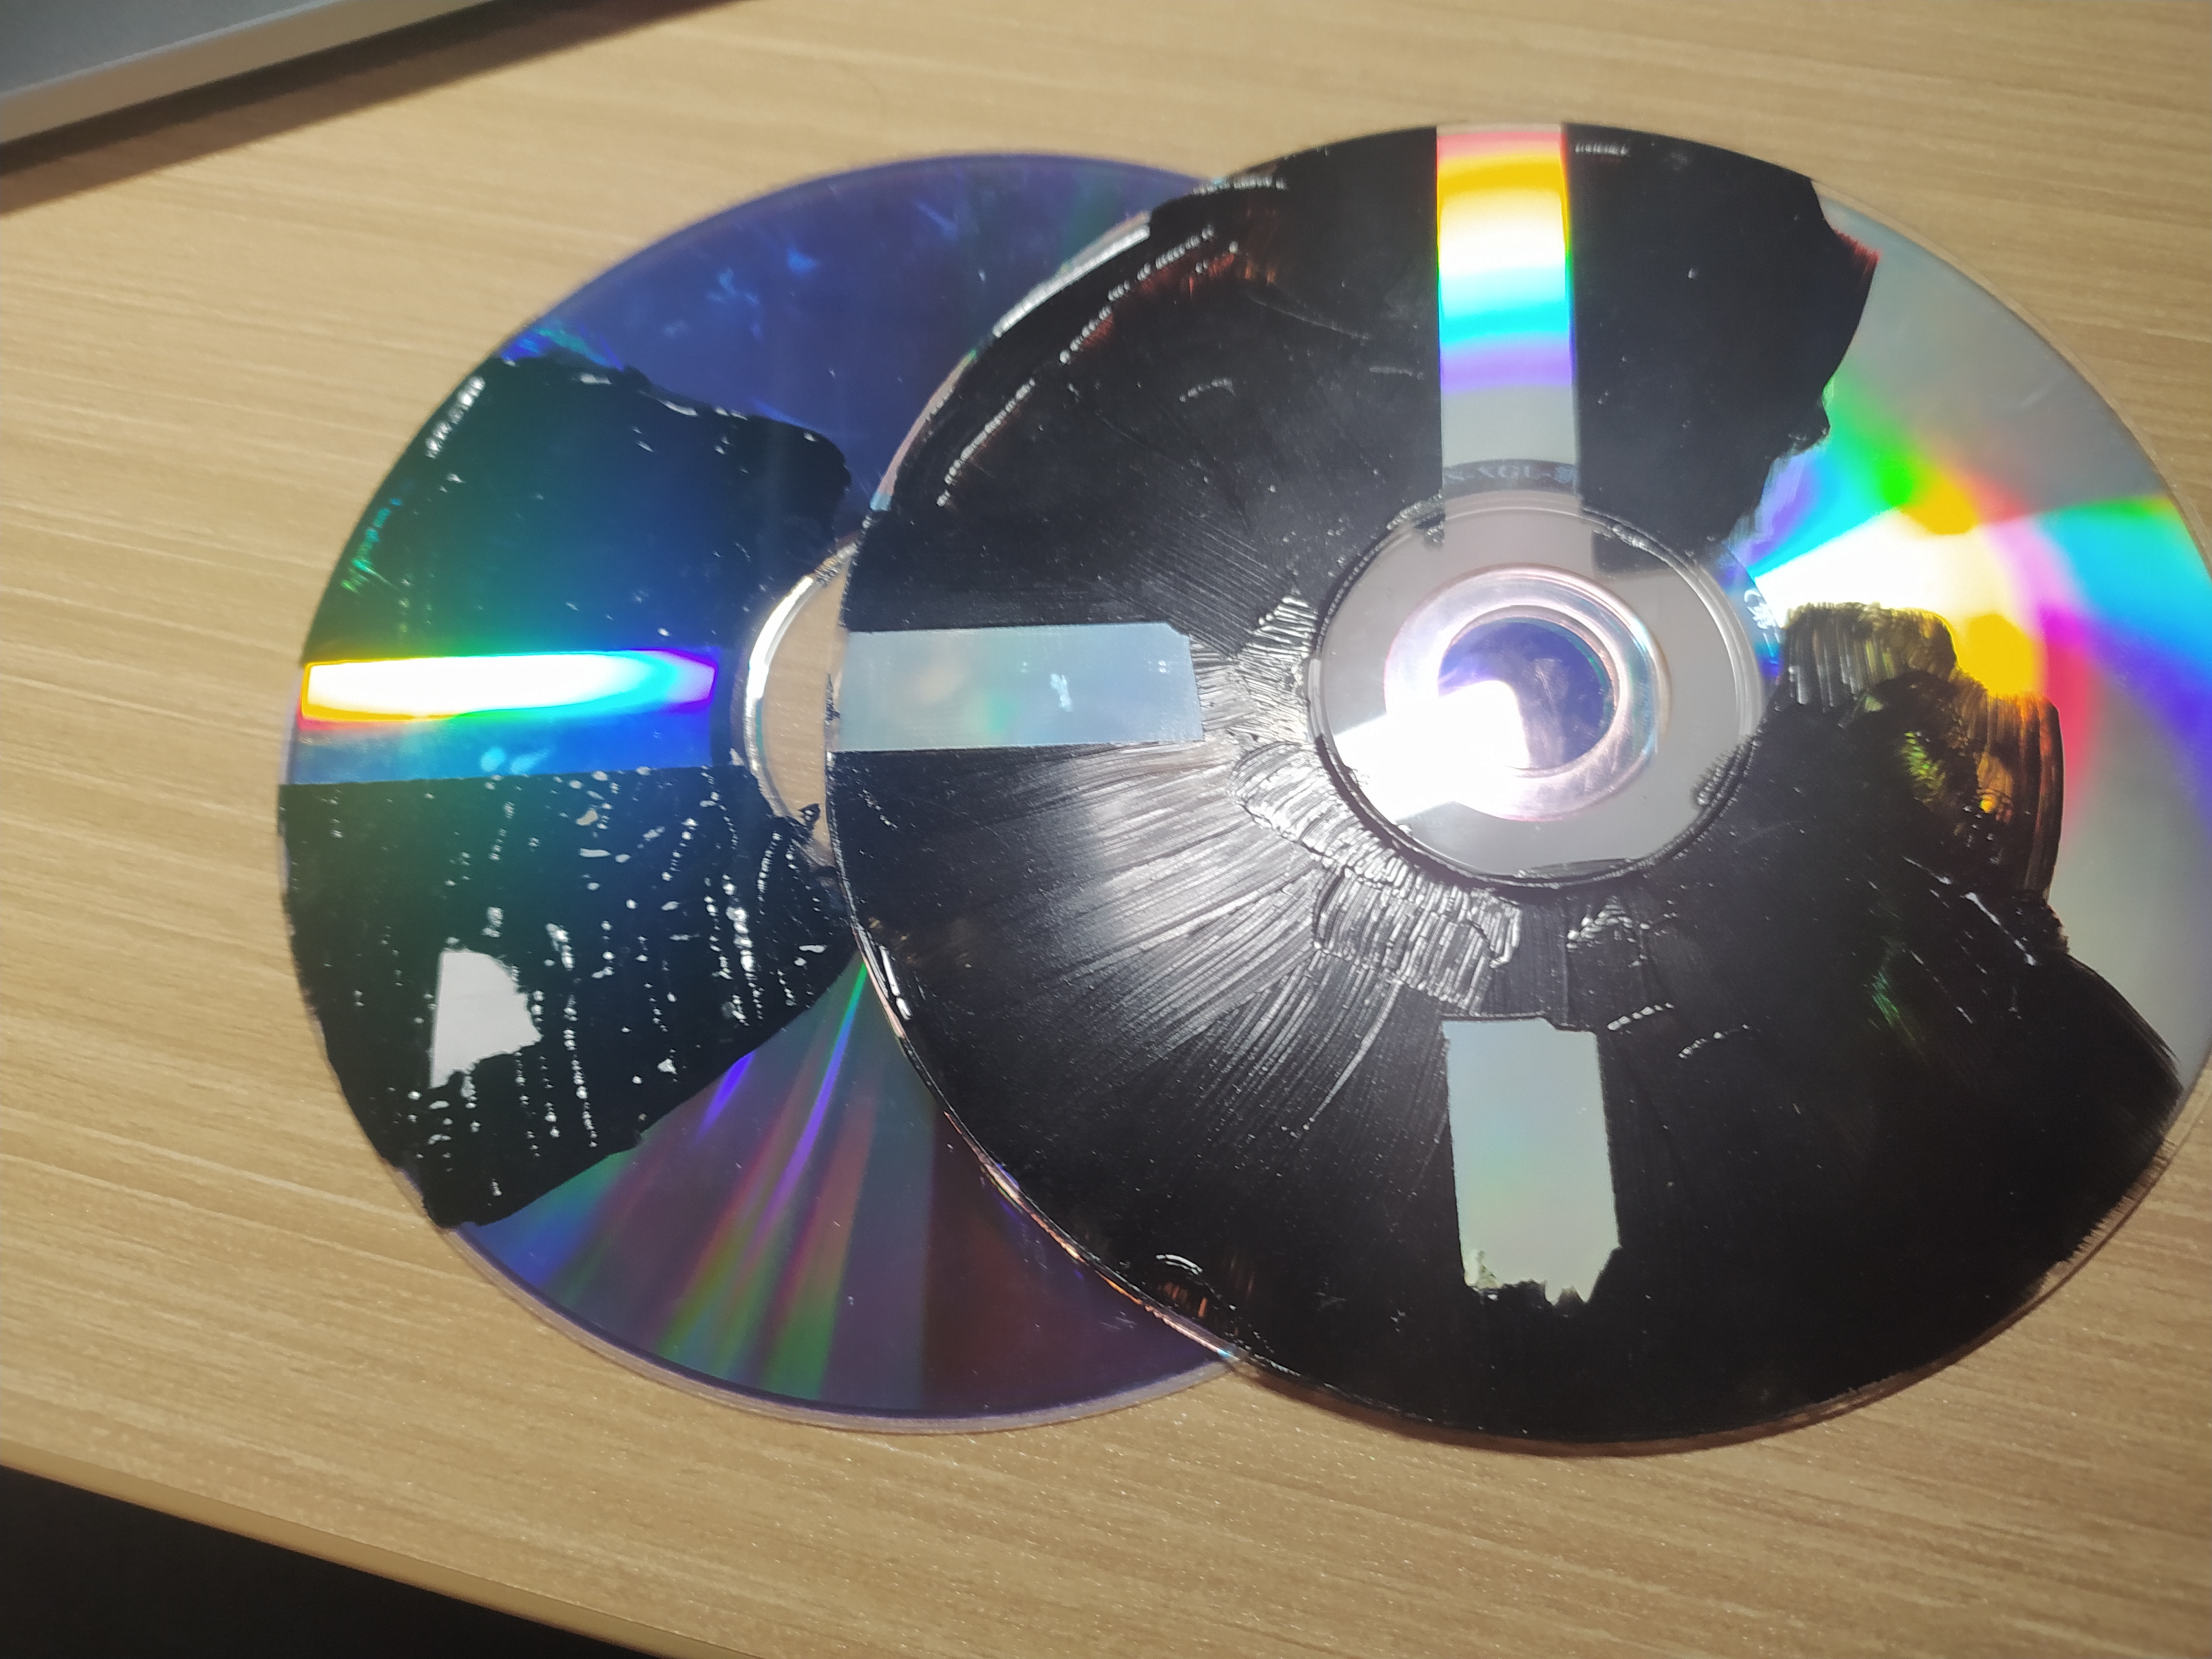
\includegraphics[scale=0.5]{2.png}
	\caption{光盘反射面光路图}
	\label{3}
\end{figure}

由于凸起部分的反射率要大于凹坑部分,且当入射角度较大,射入凹坑的光线在内部会多次反射,出射光的强度较弱,可以忽略。因此,我们只需考虑凸起部分带来的影响即可。

假设某照射点的入射角为 $\theta_i$ ,反射角为 $\theta_r$ 。在相对该照射点距离为 x 处,设新的入射角、反射角为 $\theta_i'$ , $\theta_r'$ ,设光源距离入射点距离为 $D$。如图4所示。

\begin{figure}[htbp]
	\centering
	\includegraphics[scale=0.2]{3.png}
	\caption{光盘反射面光路图}
	\label{4}
\end{figure}

此时,两束光的光程差为 $\Delta s = D(\sec\theta_i - \sec\theta_i')$ ,且满足约束条件 $D(\tan\theta_i'-\tan\theta_i) = x$ 。由于入射点较远,满足 $D \gg x$ 。因此,可近似 $\theta_i' = \theta_i + \Delta\theta$ 。由约束条件,$D\sec^2\theta_i \Delta\theta = x$ 。代入,得光程差为:

$$
\begin{aligned}
    \Delta s &= D(\sec\theta_i - \sec\theta_i')\\
             &= D\sec^2\theta_i \sin\theta_i \Delta\theta \\
             &= x\sin\theta_i
\end{aligned}
$$

反射光同理。因此,当照射点的距离差为 $x$ ,光程差满足 $\Delta s = x(\sin\theta_i - \sin\theta_r)$ 。

对于某个凸起,假设其长度为 $s$ ,记其左端点相对坐标为 0 ,相对光程差为 0。由于 $D \gg x$ 我们可以假设入射光强矢量大小在 $[x,x+\Delta x]$ 范围内近似为 $\alpha \Delta x$ ,其中 $\alpha $ 近似为常数。设入射光为单色光,角波数为 $k$ ,记 $\beta = k(\sin\theta_i - \sin\theta_r)$ 。此时,该突起上的合光强矢量为:

$$
\begin{aligned}
    \vec{E} &= \int_0^s{\alpha \exp(-i\beta x) \mathrm{d}x} \\
            &= \frac{\alpha}{i \beta}(1 - \exp(-i\beta s))  \\
            &= \frac{2\alpha}{\beta}\sin \frac{\beta s}{2}\exp(-i\frac{\beta s}{2})
\end{aligned}
$$

因此每个凸起内的衍射效应,可以等效为在 $\frac{s}{2}$ 处的一束光,即相位同凸起中心处的一束光。由于 $D \gg x$ ,因此不同凸起对于同一反射角的反射光强也近似相同。

对于不同凸起之间的衍射效应,我们将最中间的凸起编号为 0 ,相对光程差为 0。假设所有凸起编号范围为 $[-N,N]$ ,相邻凸起中心的距离为 $d$ ,设每束反射光强矢量大小均为 $E_0$ ,则合光强矢量为:

$$
\begin{aligned}
    \vec{E} &= \sum_{n = -N}^{N} E_0 \exp(-i\beta n d) \\
            &= E_0 \frac{\sin(\frac{2N + 1}{2}\beta d)}{\sin(\frac{1}{2}\beta d)}
\end{aligned}
$$

因此,总光强为:

$$
I = I_0 \frac{\sin^2(\frac{2N + 1}{2}\beta d)}{\sin^2(\frac{1}{2}\beta d)}
$$

分析该函数,如图5所示。

\begin{figure}[htbp]
	\centering
	\includegraphics[scale=0.2]{4.png}
	\caption{ $N = 4$,$\beta = 1$ 的函数图像}
	\label{5}
\end{figure}

可以看出,当 $\frac{\beta d}{2} \rightarrow m \pi (m\in\mathbb{Z})$ 时, $I\rightarrow I_0 (2N + 1)^2$ 。在附近展开,设 $\delta = \frac{\beta d}{2} - m \pi \rightarrow 0$ ,则当 $N \gg 1$ ,满足 $I \approx I_0 (2N + 1)^2 (1 -  \frac{1}{3}N^2 \delta^2)$ 。可以看出,光强在极大值点附近快速衰减。因此只有特定的方向才能观察到明显的衍射条纹。而极大值的条件为 $\frac{\beta d}{2}  = m \pi$ ,即:

$$
k(\sin\theta_i - \sin\theta_r) d = 2m \pi
$$

而角波数 $k = \frac{2\pi}{\lambda}$ ,因此代入,得到极大值条件为:

$$
\theta_r = \arcsin (\sin\theta_i - m\frac{\lambda}{d})
$$

其中,当 m = 0 ,$\theta_i = \theta_r$为满足反射定律的特殊情况。

\section{实验设计}

\subsection*{实验设备}

标准的 CD 和 DVD;一盏台灯,选用条形台灯充当线光源;直尺等测量工具;白纸若干。

\subsection*{实验方法}

为了排除环境光的干扰,我们在暗室内进行试验。我们选择桌面作为水平面,将光盘竖直放置,用光线照射  光盘平面  与  通过光盘中心的水平面  相交得到的半径区域,如图6所示。同时,我们在反射光所在一侧,平行于光盘面放置白纸,用来观察反射光的情况。

为了达到理想的效果,我们对光盘进行遮光处理,使仅有一小部分区域作为反射面。需要注意的是,该区域不宜过窄或过矮,否则反射光太弱,难以观测,会增大误差。该区域也不宜过宽,否则不能满足入射距离 $D \gg x$ 的条件,因此不可近似认为入射角处处相等,进而带来误差。该区域也不宜过高,否则在偏离该半径圆心角为 $\alpha$ 处,光栅的方向不再沿水平面,光栅的横向有效长度 $d' = d\cos \alpha$ 存在偏差,进而会带来误差。

在放置完成设备以后,调整台灯位置,控制并固定以大角度入射,并尽可能的使反射光强度明显以在纸上有清晰的图像。

为了定量的测量反射角,我们在白纸上标注了刻度,记录光盘中心的投影所在的刻度为 0,固定白纸到光盘反射面的距离。通过测量光线在白纸上的位置和光盘中心的投影的水平距离,用三角函数求出反射角度。

而为了控制入射角,我们在光盘前放置小障碍物,此时入射角即为障碍物的影子与光盘水平半径的角度。

\section{实验结果}

在实验中,我们固定入射角度 $\theta_i = 70^\circ$ ,白纸平面到光盘平面的距离为 $h = 20.0\mathrm{cm}$ ,测量色带中心位置,得到以下数据 :

\begin{table}[htbp]
    \centering
    \caption{DVD 实验数据记录表}
    \label{table1}
    \renewcommand\arraystretch{1.5}
    \tabcolsep = 1cm
    \begin{tabular}{|c|c|c|c|}
        \hline
        \multirow{2}{*}{\textbf{条纹级数 $m$}} & \multicolumn{3}{|c|}{\textbf{色带中心位置 $x/\mathrm{cm}$}}\\
        \cline{2-4} %在 2 ~ 4 行下面划线
        & \textbf{蓝色} & \textbf{绿色} & \textbf{红色} \\
        \hline
        0 & & & \\
        \hline
        1 & & & \\
        \hline
        2 & & & \\
        \hline
    \end{tabular}
\end{table}

\begin{table}[htbp]
    \centering
    \caption{CD 实验数据记录表}
    \label{table2}
    \renewcommand\arraystretch{1.5}
    \tabcolsep = 1cm
    \begin{tabular}{|c|c|c|c|}
        \hline
        \multirow{2}{*}{\textbf{条纹级数 $m$}} & \multicolumn{3}{|c|}{\textbf{色带中心位置 $x/\mathrm{cm}$}}\\
        \cline{2-4} %在 2 ~ 4 行下面划线
        & \textbf{蓝色} & \textbf{绿色} & \textbf{红色} \\
        \hline
        0 & & & \\
        \hline
        1 & & & \\
        \hline
        2 & & & \\
        \hline
    \end{tabular}
\end{table}

\section{结果讨论}




\begin{thebibliography}{30}

    \bibitem{ref1} 这是引用文献

\end{thebibliography}

\end{document}
